%# -*- coding:utf-8 -*-
\documentclass[12pt,aspectratio=169,mathserif]{beamer}		
%\documentclass[12pt,mathserif]{beamer}		
%设置为 Beamer 文档类型,设置字体为 10pt,长宽比为16:9,数学字体为 serif 风格
%\documentclass{beamer}

%%%%-----导入宏包-----%%%%
\usepackage{gdut}			%导入 GDUT 模板宏包
\usepackage{ctex}			%导入 ctex 宏包,添加中文支持
\usepackage{amsmath,amsfonts,amssymb,bm}   %导入数学公式所需宏包
\usepackage{color}			 %字体颜色支持
\usepackage{graphicx,hyperref,url}
\usepackage{metalogo}	% 非必须
\usepackage{multicol}
%% 上文引用的包可按实际情况自行增删
%%%%%%%%%%%%%%%%%%	


\beamertemplateballitem		%设置 Beamer 主题

%%%%------------------------%%%%%
\catcode`\。=\active         %或者=13
\newcommand{。}{.}				
%将正文中的“。”号转换为“.”。中文标点国家规范建议科技文献中的句号用圆点替代
%%%%%%%%%%%%%%%%%%%%%

% Bibliography settings 参考文献设置
\usepackage[style=ieee]{biblatex}
\setbeamertemplate{bibliography item}[text]


%\tiny\scriptsize\footnotesize\small\normalsize\large\Large\LARGE\huge\Huge   这些是调整字体大小的命令。

%%%%----首页信息设置----%%%%
\title[ 广工 Beamer 模板]{广东工业大学 Beamer 模板}
\subtitle{——这里是副标题}			
%%%%----标题设置


\author[Zheng Xue]{
   \large 薛\quad 拯 \\\medskip
  {\small \url{xuezheng@mail2.gdut.edu.cn}} \\
  {\small \url{http://www.gdut.edu.cn/}}
  }
%%%%----个人信息设置
  
\institute[IOPP]{
   \normalsize 广东工业大学信息工程学院 \\ 
  电子与通信工程}
%%%%----机构信息

\date[Dec. 12 2020]{
  2020年12月12日}
%%%%----日期信息
  
\begin{document}

%----------------------------------------------------------------------------------------
%	TITLE PAGE
%----------------------------------------------------------------------------------------

\begin{frame}
\titlepage
\end{frame}				%生成标题页

\begin{frame}{目录} % Table of contents slide, comment this block out to remove it
%\tableofcontents % Throughout your presentation, if you choose to use \section{} and \subsection{} commands, these will automatically be printed on this slide as an overview of your presentation
\tableofcontents[sectionstyle=show,subsectionstyle=show/shaded/hide,subsubsectionstyle=show/shaded/hide]

\end{frame}

\AtBeginSection[]
{
  \begin{frame}
    \frametitle{目录}
    \tableofcontents[currentsection]
  \end{frame}
}


%----------------------------------------------------------------------------------------
%	PRESENTATION SLIDES
%----------------------------------------------------------------------------------------

%------------------------------------------------
\section{介绍}% Sections can be created in order to organize your presentation into discrete blocks, all sections and subsections are automatically printed in the table of contents as an overview of the talk
%------------------------------------------------

\begin{frame}
  \frametitle{介绍}

  \begin{itemize}
    \item {编译方式}
	    \begin{itemize}
	    	\item  推荐使用 Overleaf
	    	\item 使用 \XeLaTeX 编译
	    \end{itemize}
    \item 请参考 \LaTeX 和 Beamer 用户文档 
    
    \item 行内数学公式示例 $\sin^2 \theta + \cos^2 \theta = 1$
    \item {行间数学公式示例 \begin{equation}
	    y_{1}=\int \sin x\, {\rm d}x
    \end{equation}	 }   
  \end{itemize}
\end{frame}
%------------------------------------------------

%------------------------------------------------
\section{内置环境}
%------------------------------------------------

\begin{frame}
  \frametitle{内置环境}
	\begin{block}{Slides with \LaTeX}
	    Beamer offers a lot of functions to create nice slides using \LaTeX.
	  \end{block}
	
	  \begin{block}{The basis}
	    内部使用以下主题
	    \begin{itemize}
	      \item split
	      \item whale
	      \item rounded
	      \item orchid
	    \end{itemize}
	  \end{block}
\end{frame}
%------------------------------------------------
\begin{frame}
  \frametitle{带数字列表}
	 \begin{enumerate}
	    \item This just shows the effect of the style
	    \item It is not a Beamer tutorial
	    \item Read the Beamer manual for more help
	    \item Contact me only concerning the style file
	  \end{enumerate}
\end{frame}
%------------------------------------------------
\begin{frame}{块并列}
\begin{columns}
\begin{column}{0.5\textwidth}
\begin{block}{block1}
%\footnotesize{
\begin{enumerate}
        \item item1
        \begin{itemize}
            \item  item1.1
        \end{itemize}
        \item item2
        \begin{itemize}
            \item item2.1
        \end{itemize}
        \item item3
        \begin{itemize}
            \item item3.1
        \end{itemize}
\end{enumerate}    
%}    
\end{block}
\end{column}
\begin{column}{0.5\textwidth}
\begin{block}{block2}
%\footnotesize{
\begin{enumerate}
        \item item1
        \begin{itemize}
            \item  item1.1
        \end{itemize}
        \item item2
        \begin{itemize}
            \item item2.1
        \end{itemize}
        \item item3
        \begin{itemize}
            \item item3.1
        \end{itemize}
\end{enumerate}    
%}    
\end{block}
\end{column}
\end{columns}
\end{frame}
%------------------------------------------------

\begin{frame}{图片}
    \begin{minipage}{0.4\linewidth}
\begin{figure}[h]
            \centering
            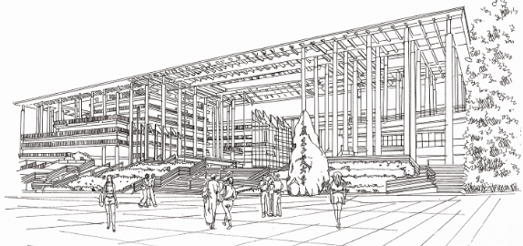
\includegraphics[height=.4\textheight]{res/GDUT-gate.png}
            \caption{GDUT}
 \end{figure}
    \end{minipage}\hspace{0.3cm}
    \begin{minipage}{0.45\linewidth}
    \begin{figure}[h]
            \centering
            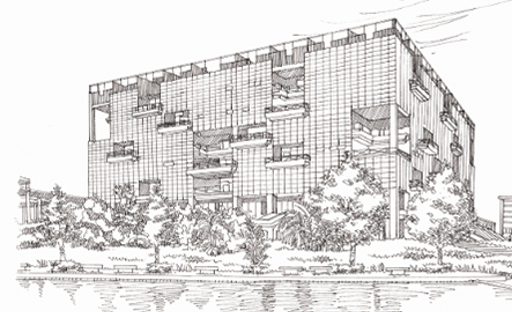
\includegraphics[height=.4\textheight]{res/GDUT-library.png}
            \caption{GDUT}
 \end{figure}   
    \end{minipage}%\hspace{0.1cm}
\end{frame}
%------------------------------------------------

\begin{frame}[t]{块中多图}
\begin{small}
\begin{block}{多图比较与分析}
\begin{minipage}{0.5\linewidth}
\begin{figure}[h]
            \centering
            
\includegraphics[height=.2\textheight]{res/GDUT-logo.png}
            \caption{GDUT}
 \end{figure}
    \end{minipage}\hspace{0.1cm}
    \begin{minipage}{0.45\linewidth}
    \begin{figure}[h]
            \centering
            
\includegraphics[height=.2\textheight]{res/GDUT-logo_black.png}
            \caption{GDUT}
 \end{figure}   
    \end{minipage}\hspace{0.1cm}
    %\medskip
        \begin{minipage}{0.5\linewidth}
    \begin{figure}[h]
            \centering
            
\includegraphics[height=.2\textheight]{res/GDUT-logo_white.png}
            \caption{GDUT}
 \end{figure}   
    \end{minipage}\hspace{0.4cm}
\begin{minipage}{0.4\linewidth}
\begin{block}{}
\begin{itemize}
\scriptsize{
\item ****************
\item ****************
\item ****************
}
\end{itemize}
\end{block}
\end{minipage}
\end{block}
\end{small}
\end{frame}
%------------------------------------------------


%------------------------------------------------
\section{结论}
%------------------------------------------------
\begin{frame}
\subsection{  \frametitle{结论}}

  \begin{itemize}
    \item Easy to use
    \item Good results
  \end{itemize}
\end{frame}
%------------------------------------------------

%------------------------------------------------
\section{参考文献}
%------------------------------------------------
\begin{frame}
\frametitle{参考文献}
\begin{block}{}
\begin{minipage}{1\linewidth}
\scriptsize{
\begin{thebibliography}{99} % Beamer does not support BibTeX so references must be inserted manually as below
\bibitem{1} R. Sun, Y. Wang, L. Lyu, N. Cheng, S. Zhang, T. Yang, and X.Shen,“Delay-oriented caching strategies in d2d mobile networks,” \emph{IEEE Trans. Veh. Technol.}, vol. 69, no. 8, pp. 8529–8541, Aug. 2020.
\item Z. Su, Y. Hui, Q. Xu, T. Yang, J. Liu, and Y. Jia,“An edge caching scheme to distribute content in vehicular networks,” \emph{IEEE Trans. Veh. Technol.}, vol. 67, no. 6, pp. 5346–5356, Jun. 2018.
\item Q. Xu, Z. Su, Y. Wang, and K. Zhang,“Secure edge caching for layered multimedia contents in heterogeneous networks,” in \emph{Proc. IEEE Global Commun. Conf.}, Waikoloa, HI, USA, Dec. 2019, pp. 1–6.
\item B. Hu, L. Fang, X. Cheng, and L. Yang,“In-vehicle caching (iv-cache) via dynamic distributed storage relay ($d^2$sr) in vehicular networks,” \emph{IEEE Trans. Veh. Technol.}, vol. 68, no. 1, pp. 843–855, Jan. 2019.
\item C. Liu, K. Liu, S. Guo, R. Xie, V. C. S. Lee, and S. H. Son,“Adaptive offloading for time-critical tasks in heterogeneous internet of vehicles,” \emph{IEEE Internet Things J.}, vol. 7, no. 9, pp. 7999–8011, Sep. 2020.
\item J. Chen, H. Wu, P. Yang, F. Lyu, and X. Shen,“Cooperative edge caching with location-based and popular contents for vehicular networks,” \emph{IEEE Trans. Veh. Technol.}, vol. 69, no. 9, pp. 10291-10305, Jun. 2020.
\end{thebibliography}
}
\end{minipage}
\end{block}
\end{frame}
%------------------------------------------------


%------------------------------------------------
\section{}

\begin{frame}
\begin{block}{Ending}
\Huge{\centerline{\emph{Thanks for Your Attention!}}}
\Huge{\centerline{\emph{Q \& A ?}}}
\end{block}

\end{frame}
%------------------------------------------------

\end{document}